\chapter{Alignment of the CMS Silicon Tracker}
\newcommand{\MPII}{\textsc{millepede}-II\xspace}
\newcommand{\HIPPY}{\textsc{HipPy}\xspace}
\newcommand{\MINRES}{\textsc{MinRes}\xspace}

The CMS silicon tracker is the largest in the world, both in terms of surface area and number of sensors.
In order to harness its exceptional resolution, a precise knowledge of the position and orientation of the modules is necessary.
During the installation, the mechanical alignment of the modules resulted in a precision of O(100\mum),
which is much larger than the design hit resolution of the modules of O(10\mum).

Consequently, an additional refinement addressing the positional accuracy, orientation, and surface deformations of the sensors becomes imperative.
This refinement, commonly denoted as the tracker alignment, is characterized by the derivation of a set of parameters known as the tracker alignment constants.
These constants, which amount to around $200\,000$, are used during the track reconstruction to determine the true position of the hits.

Changes in the environment such as temperature variations and the ramping of the magnetic field induce movements in the tracker structures,
motivating regular updates of the alignment constants to maintain the target precision.
The method used in CMS to derive the constants consists in performing track fits with the corresponding track parameters unconstrained.

\paragraph{Hierarchical alignment\\}
The alignment parameters of the CMS tracker are organized in a hierarchy that follows the one of the modules themselves (see Figure \ref{fig:tracker_hierarchy}).

Each element of the hierarchy has its own six parameters (3 translations and 3 rotations).
This adds redundant degrees of freedom, since the movements of the large structures can be equivalently expressed by shifts of elements within their sub-hierarchies.
The redundancy is removed by linear equality constraints,
imposed on the original equation system with Lagrange multipliers
or by elimination.
This treatment of alignables allows the fitting of only the large mechanical structures with varying granularity,
which is especially useful when the number of track is limited, \eg when restarting data-taking after a commissioning period.

\section{Track-based alignment}
The track-based alignment consists in the determination of the correct alignment constants using the measured hits and reconstructed tracks.
The alignment parameters $\vec{p}\,$ are fitted by minimizing the following $\chi^2$ function:

\begin{equation}
  \chi^2(\vec{p}, \vec{q}\,) \sum_j^{\rm tracks} \sum_i^{\rm hits} \left( \frac{m_{ij} - f_{ij}(\vec{p}, \vec{q_j})}{\sigma_{ij}^{m}} \right)
\end{equation}

where
\begin{itemize}
  \item The $\vec{p}$ are the (global) alignment parameters.
  \item The $\vec{q}$ are the parameters of the tracks (\eg the track curvature or the deflection at a given detector layer).
    The $\vec{q_j}$ are the parameters of the $j$-th track.
  \item The $m_{ij}$ are the measurements (hits).
  \item The $f_{ij}$ are the predicted measurements using the track parameters and the alignment constants.
  \item The $\sigma^m_{ij}$ are the uncertainties of the measurements, due to local hit resolution and alignment uncertainty.
\end{itemize}

The alignment procedure allows for a variable subset of the parameters to be fitted, while keeping the other fixed.
This strategy is used for example when resuming data taking after commissioning or a magnet cycle, where initially only the high level structures are aligned,
leading to only 36 parameters.

The fitting procedure extracts the best values for the $\vec{p}\,$ regardless of the (potentially millions of) track parameters $\vec{q_j}\,$,
thus allowing alignment campaigns with large datasets and many degrees of freedom.
This is achieved by linearising the $\chi^2(\vec{p_0}\,+\Delta p, \vec{q_0}\,+\Delta q)$ as deviations from a previous set of alignment parameters.
Its minimization can be expressed by a set of linear equations containing the measurements and the derivatives in the alignables or track parameters,
and treated like a matrix inversion problem:
\begin{equation}
  \label{eq:alignment_full_matrix}
  C \times \binom{\Delta\vec{p}}{\Delta\vec{q}} = \vec{b}
\end{equation}
Employing block matrix algebra it is possible to factorize the problem such that only a sub-matrix involving the $\Delta p$ has to be inverted,
while maintaining all the correlations from the track parameters~\cite{blobel2002new}.
Equation~\ref{eq:alignment_full_matrix} is reduced to:
\begin{equation}
  \label{eq:alignment_reduced_matrix}
  C' \times \Delta\vec{p} = \vec{b'}
\end{equation}
The $C'$ and $\vec{b'}$ have a significantly smaller sizes than $C$ and $\vec{b}$,
of the order of $\mathcal{O}(10\,000)$.

\section{Alignment algorithms}
Two independent track-based alignment algorithms are used by the CMS Collaboration~\cite{CMS-TRK-20-001}, \MPII and \HIPPY.
The former also performs a global matrix inversion, while the latter neglects the blocks
relating the global alignables to the track parameters and iterates to improve the approximation.
Both are maintained and used, thus enabling cross-checks.

\subsection[Millepede-II]{\MPII}
The \MPII algorithm~\cite{blobel2002new,Blobel:2006yh,terascale-wiki} has been discussed in the context of CMS in Reference~\cite{CMS-TRK-11-002}.
In addition to CMS, The Belle~II experiment~\cite{PROC-CTD19-098} is also a main user.
The algorithm consists of two steps:
\begin{description}
  \item[\textsc{Mille}] This is integrated into the experiment-specific track-fitting software.
    Calculates and stores the track residuals with errors and the derivatives of the
    track (local) and module (global) parameters.
    The track fitting method must fit all the hits simultaneously and provide the full covariance matrix.
    The solution is based on the general broken lines method~\cite{Blobel_2011}.
  \item[\textsc{Pede}] This is an independent Fortran program that solves the linear equation system needed for the alignment.
    It uses the \textsc{Mille} output to perform the local fits and construct the global matrix $C'$ from Equation~\ref{eq:alignment_reduced_matrix}.
    An overview of the solution methods that are implemented is given in Table~\ref{tab:MP_solvers}.
\end{description}

\begin{table}
  \caption{Comparison of the solution methods implemented in \MPII.
  The computation time is reported as a function of the number of parameters $n$ and the number of iterations $n_{\rm it}$ if applicable.}
  \label{tab:MP_solvers}
  \centering
  \begin{tabular}{l l l l}
    \toprule
    Method                             & Computing time              & Solution type & Error calculation \\
    \midrule
    Gauss-Jordan inversion             & $\sim n^3$                  & Exact         & Yes \\
    Cholesky decomposition             & $\sim n^3$                  & Exact         & Skipped \\
    \MINRES \cite{Choi_2011,Choi_2014} & $\sim n^2 \times n_{\rm it}$ & Approximate   & No \\
    \bottomrule
  \end{tabular}
\end{table}

\subsection[HipPy]{\HIPPY}
Based on the hits-and-impact-points algorithm~\cite{karimaki2003sensor,CMS-NOTE-2006-018}
and improved for the BaBar alignment~\cite{BaBar_alignment},
it has been used extensively during the tracker commissioning
and CMS startup in \Run1~\cite{CMS-NOTE-2009-002}
and further improved in \Run2.
The improved algorithm is named hits-and-impact-points-past-year-1 (\HIPPY).

Unlike \MPII, it is local in that the alignment of each sensor is determined independently of the others.
The tracks are fitted, after applying the corresponding constraints,
with a given set of alignment conditions.
The $\chi^2$, expressed as a function of the alignment parameter, is minimized on a per-module basis.
Different weights can be assigned to different types of tracks,
and a new set of alignment conditions is computed and passed back to the track fitting.
The process is repeated until convergence is reached.

One disadvantage is that multiple iterations,
ranging from a few dozens to a hundred,
each requiring CPU-intensive track fits,
are required to solve correlations between alignables.
The advantages include the native integration with CMS software, providing features such as
the CMS Kalman filter code for track propagation
and the implementation of constraints such as mass or vertex constraints.
Each iteration of the algorithm is a very simple application of a small matrix inversion.
This simplicity and dependence on the CMS software makes the \HIPPY algorithm complementary to \MPII.

\section{Datasets}
Different types of datasets are generally used for the alignment.
The main benefit of a diverse set of tracks is that each track topology correlates a different set of alignables.

The main datasets are:
\begin{itemize}
\item \textbf{collisions}
  \begin{itemize}
  \item minimum bias, a sample of randomly chosen events passing the L1 trigger (Section \ref{sec:L1trigger});
  \item isolated muons: events passing one of the single muon HLT triggers with isolation cuts on a cone of radius $\DR = 0.1$;
  \item dimuon resonances: pairs of muons with a mass close to the \PZ or $\Upsilon$ %% \PGU looks too much like a Y
  \end{itemize}
\item \textbf{cosmic muons:}
  \begin{itemize}
  \item Cosmic RUns at ZEro Tesla (CRUZET), before magnet ramp up (no \pt requirements since it is not measured);
  \item Cosmic Runs At Four Tesla (CRAFT), after the magnet ramp-up;
  \item Interfill cosmics, taken in dedicated runs between LHC fills, with conditions similar to CRAFT;
  \item Cosmics During Collisions (CDC);
  \end{itemize}
\end{itemize}
All of the tracks have a minimum \pt requirement, ranging from 1 to 5\GeV depending on the dataset.

Collisions datasets contain tracks propagating outwards from the interaction point, which correlate the modules radially.
These datasets contain several million tracks which are essential for a full module level alignment.

CMS has dedicated algorithms for the reconstruction of cosmic tracks both for commissioning and calibration.
CRUZET and CRAFT are available for alignment before the start of LHC collisions, to provide an alignment after a shutdown period.
Cosmic ray muons cross the whole detector, connecting modules located in the top and bottom halves.
This is fundamental to constrain several types of systematic distortions.

\section{Systematic misalignments}
Systematic shifts of the assumed position of the modules with respect to the real ones
are called systematic misalignments of the tracker geometry. They
may cause biases in the track reconstruction and negatively impact the physics performance.

A noteworthy class of misalignment is composed by the \textit{weak modes}.
They are transformations that do not affect significantly the $\chi^2$ of the tracks,
and are caused by a lack of constraints in the alignment fit.
While these shifts do not degrade the tracking performance,
they may affect certain topologies and correlations among tracks that are important for physics measurements.

\subsection{Validation of misalignments}
To check the quality of a set of alignment constants and the effect of misalignments,
measurements of several variables that have known values under perfectly aligned conditions are carried out.

\subsubsection{Geometry comparison} % GC
The geometry produced by the alignment is compared with a reference geometry,
such as the one used as a starting point for the procedure or the ideal conditions.
This serve as a guide to help visualize the effect of the procedure
and may permit to notice certain known nonphysical distortions.

The global shift and rotation of large structures are removed and the module displacements
$\Delta z$, $\Delta r$ and $\Delta \phi$, as well as the rotations,
are plotted as function of $z$, $r$ and $\phi$.

\subsubsection{Cosmic ray muon track} % MTS
The upper and lower portions of cosmic ray muon tracks are reconstructed separately,
and the two sets of track parameters are compared at the point of closest approach to the beamline.
The two halves should have the same parameters, while systematic differences suggest a misalignment.

Cosmic ray and collision tracks have different topologies, so distortions that appear as
weak modes in collision may be constrained with cosmic tracks.
In particular they connect the top and bottom halves of the detector in a single track,
which is not possible with collisions, and help constrain the z position of the modules.
Since cosmic ray muon tracks are collected even before the start of the collisions,
this validation is and early tool in the commissioning of the detector before the start of LHC operations.

\subsubsection{Dimuon validation} % Zmumu
The reconstructed invariant mass of $X \to \PGm\PGm$ should not depend
on the direction of the muons within the detector.
Biases in the mass distribution of a known resonances suggest a systematic misalignment. %% like $\PZ$ or $\JPsi$
\PZ bosons are especially useful since they are often produced with a small boost
resulting in two muons that cross opposite ends of the tracker.

The reconstructed mass in each event is placed into a bin depending on the $\eta$ and $\phi$ of the muons.
The mass distribution of each bin is then fit with a Gaussian function and its mean recorded.
%% Profiles in $\eta$ and $\phi$ of the fitted mean invariant mass are constructed.
Misalignment in the tracker may be detected if the mean reconstructed mass strays from the expected value of 91.2\GeV,
either uniformly or as a function of $\eta$ and $\phi$.
This validation requires a sufficiently large sample of $\PZ \to \PGm\PGm$ events
and is therefore useful in in stable operating conditions.

\subsubsection{Track-vertex impact parameter} % PV
\label{sec:TkAl_PV}
The resolution of the reconstructed vertex position is driven by the pixel detector
since it is the closest to the interaction point~\cite{CMS-TRK-11-002}.
This method is based on the study of the distance between the track and the vertex,
the latter reconstructed without the track under scrutiny (unbiased track-vertex residual).
The distribution of the unbiased track-vertex residuals in the transverse ($d_{xy}$) and longitudinal ($d_z$)
plane is studied in bins of track azimuthal angle and pseudorapidity.
Random misalignments of the modules affect only the resolution of the track-vertex residual,
increasing the width of the distribution, but without biasing its mean.
Systematic movements of the modules will bias the distribution
in a way that depends on the nature and size of the misalignment and the selected tracks.

\section{Personal contribution to the alignment group}
As part of the Tracker Alignment group, I executed several alignment campaigns and validated their performance on observables of interest,
both for the commissioning of the detector after the Long Shutdown 2 (2019--2022)
and for routine alignment during the \Run3 data-taking.
The derivation of the alignment conditions is always a group effort.
Nevertheless, my contributions include the derivation of the alignment used for the re-reconstruction of the 2022 data and its validation,
the alignment used for the 2022 Heavy Ion collisions,
and the derivation of preliminary alignment candidates for the startup of proton-proton run in 2023.

A representative result of the alignment effort is shown in Figure~\ref{fig:TkAl2023},
which compares the performance of different geometries
using the track-vertex impact parameter validation described in Section~\ref{sec:TkAl_PV}.
The performance is evaulated using a sample of collision events collected by the CMS detector at full magnetic field (3.8\unit{T})
during pp collisions data taking at $\sqrt{s} = 13.6\TeV$ in 2023, selected online through minimum bias triggers~\cite{CMS-DP-2023-039}.
The dataset used in the validation is orthogonal to the one used for the derivation of the alignment constants.

\begin{figure}
\subfigure [] {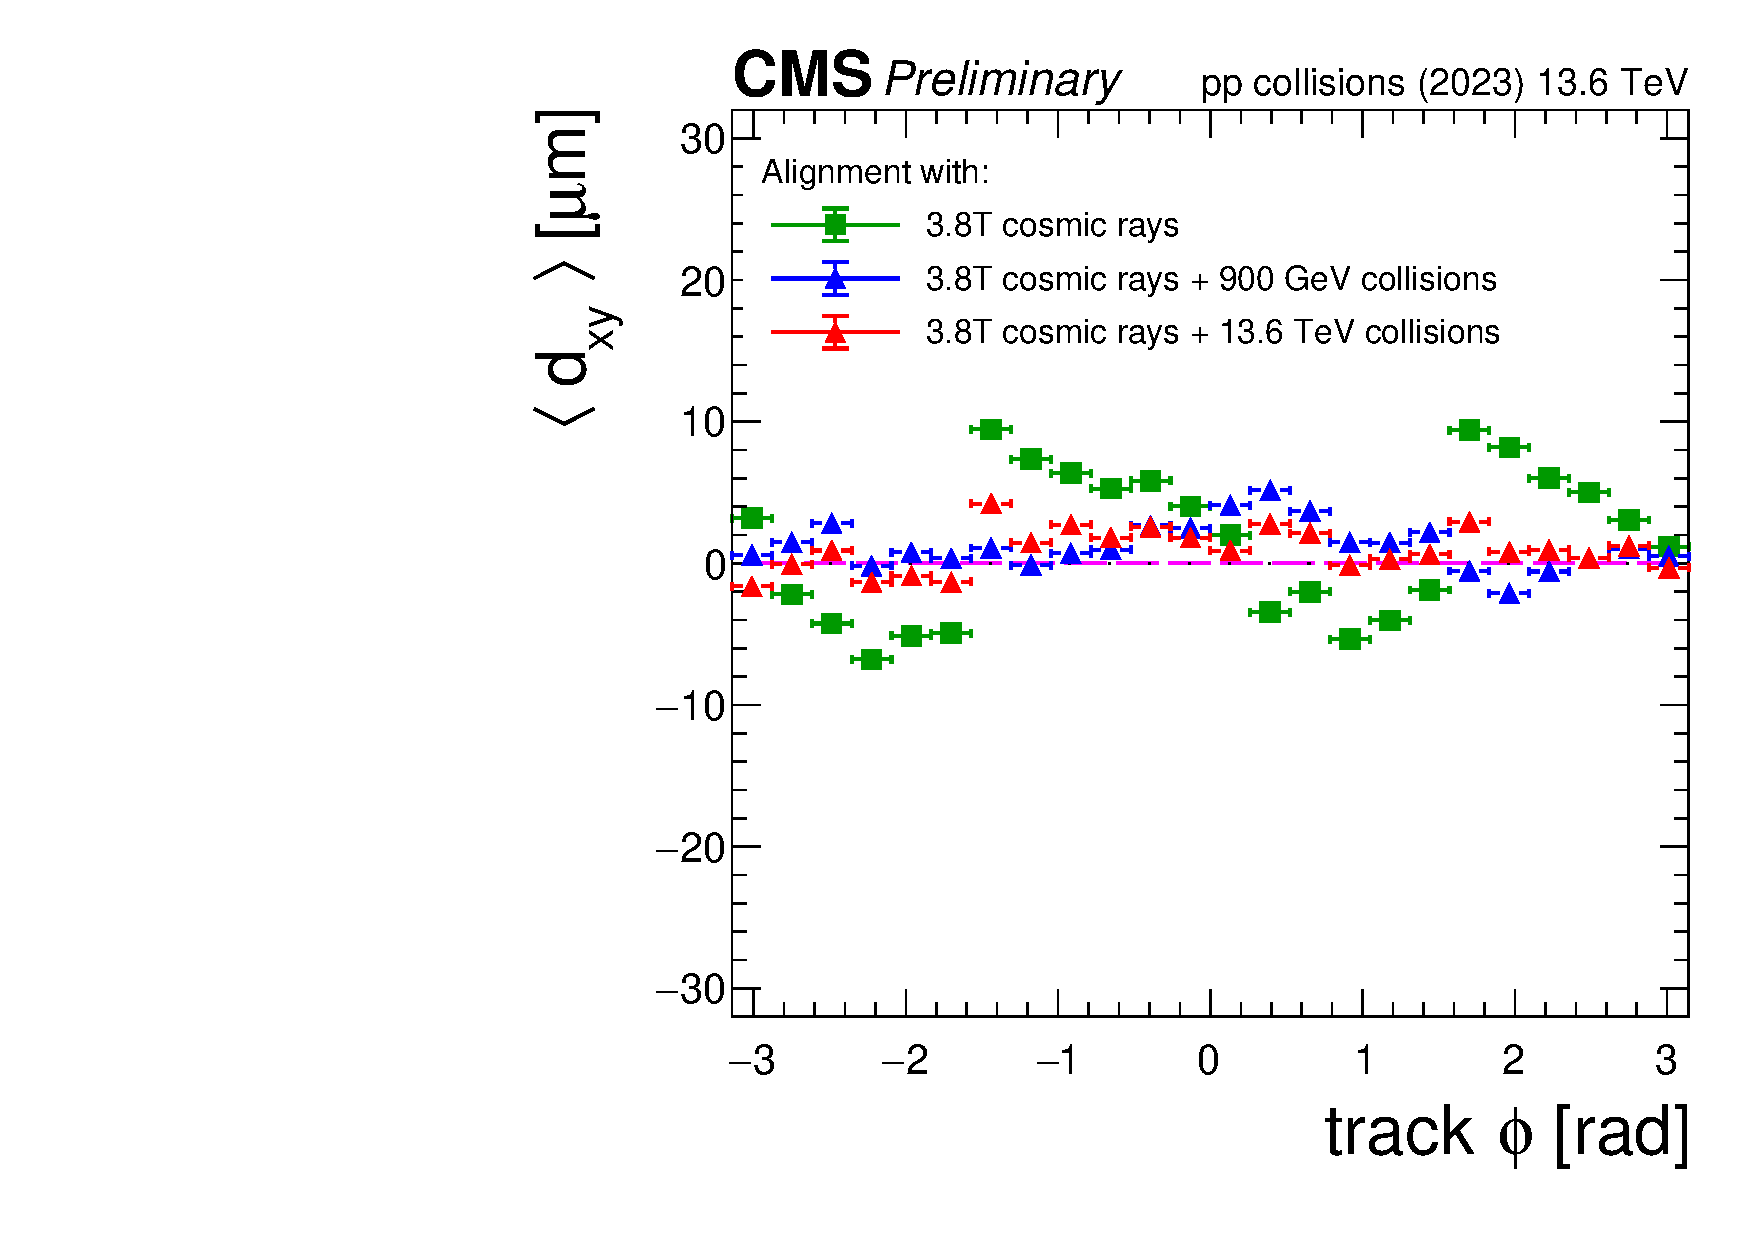
\includegraphics[width=.5\textwidth]{Figures/TkAl2023/dxyPhiBiasCanvas.pdf}}%
\subfigure [] {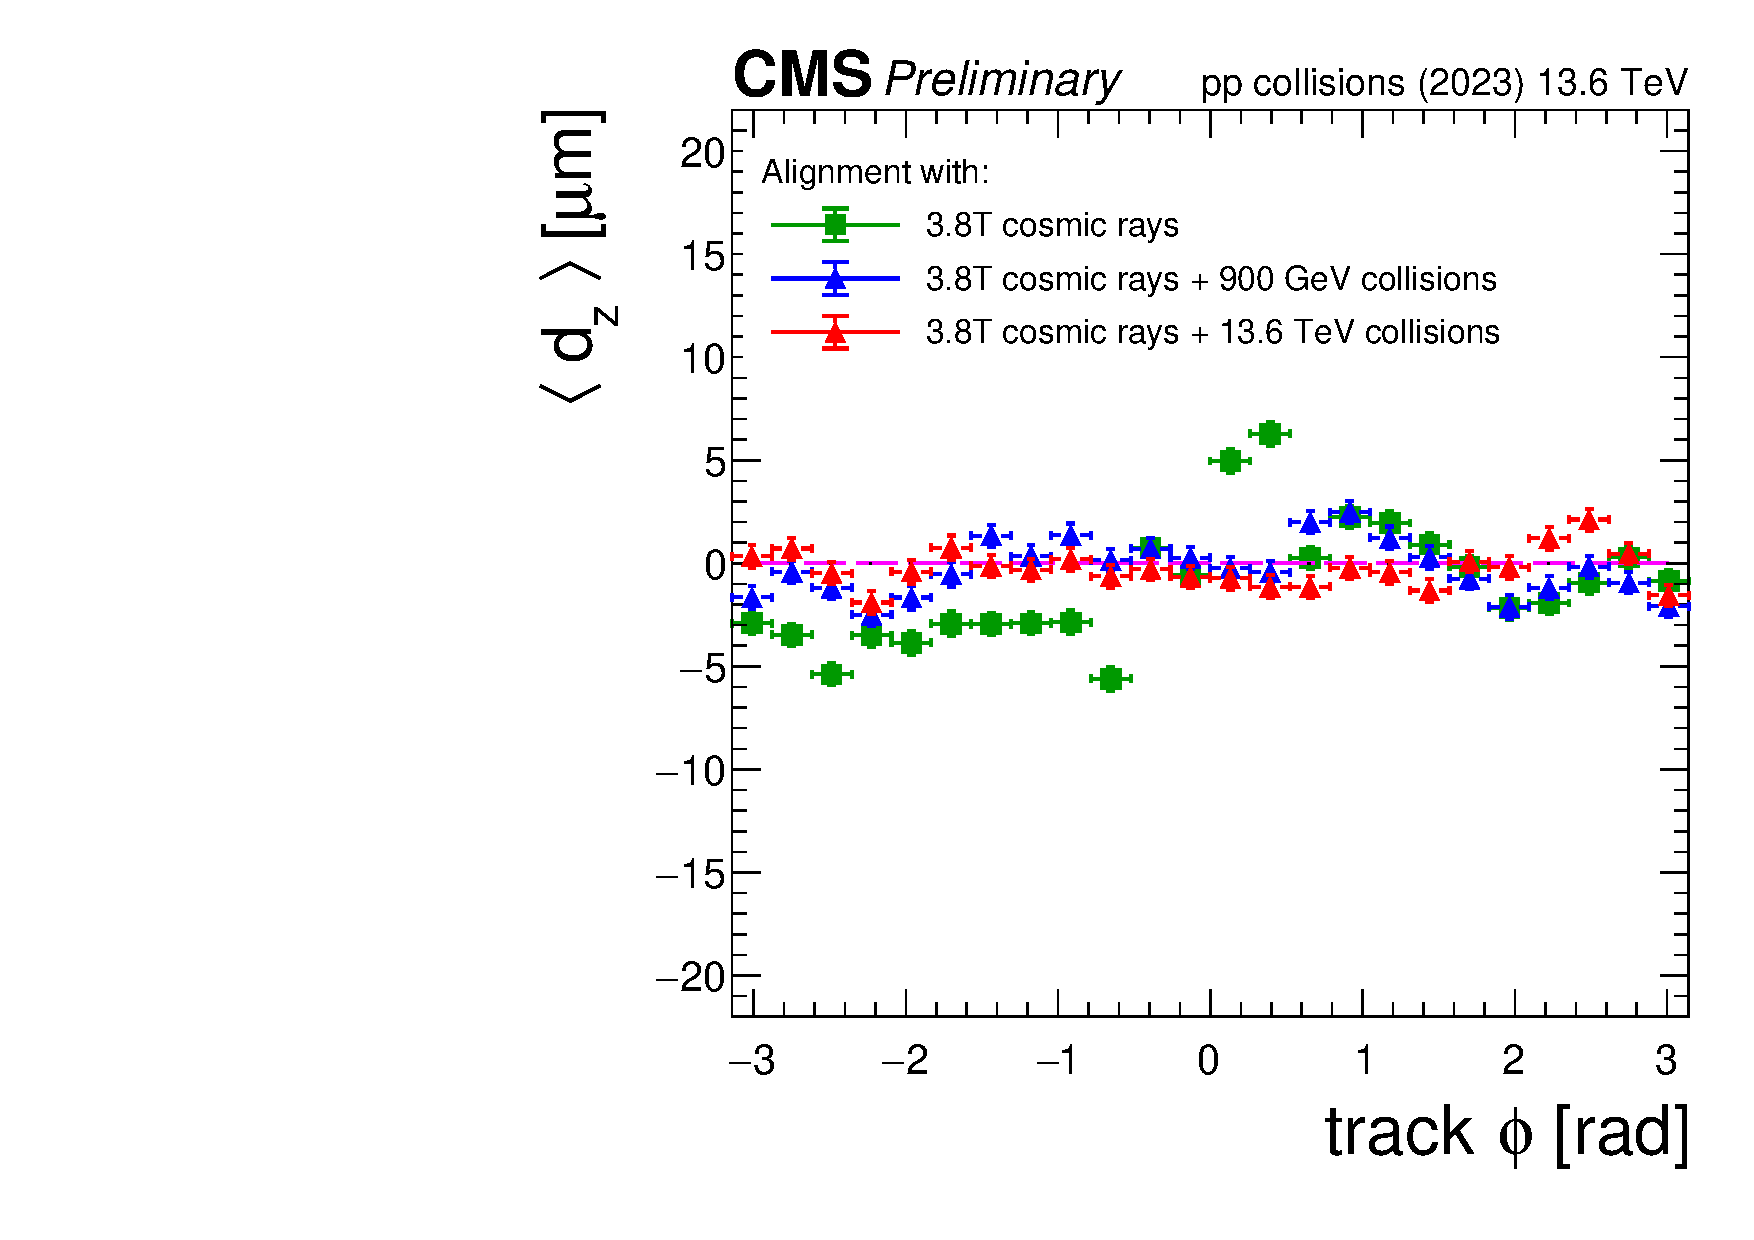
\includegraphics[width=.5\textwidth]{Figures/TkAl2023/dzPhiBiasCanvas.pdf}}
\caption{The distance in the longitudinal ($d_{xy}$, left) and transversal ($d_z$, right) directions
  of the tracks at their point of closest approach to a refit unbiased primary vertex is studied in bins of track azimuthal angle.
  The performance of the alignment obtained using 3.8\unit{T} cosmic rays (green) is compared to the alignment constants
  derived using cosmic ray and pp collision tracks collected at $\sqrt{s} = 900\GeV$ (blue) and $\sqrt{s} = 13.6\TeV$ (red).
  The residual deviations from the ideal case (purple dashed line, mean of 0) show the typically achieved precision of the alignment.
  Vertical error bars represent the statistical uncertainty due to the limited number of tracks, which can be smaller than the size of the markers~\cite{CMS-DP-2023-039}.
}
\label{fig:TkAl2023}
\end{figure}

I am also the maintainer of the software tool used to extract the position of the barycentre of the silicon pixel detector from a set of alignment constants.
The usage of this tool, which is under my responsibility, is instrumental for
the production of Monte Carlo samples of physics processes, since this point is the origin of the coordinate system in simulations,
and to monitor the position of the interaction region of the LHC beams (beamspot),
which is important to avoid excessive radiation-induced damage of the pixel detector itself.
